\chapter{Practical Implementations of DevOps Tools in Real World Application}

This chapter explores the practical implementations of DevOps tools in real-world applications, focusing on ensuring ethical compliance in regulated industries.
\begin{enumerate}
    \item We begins by discussing the relevance of Linux commands in DevOps implementation and server management. Also we give a list of all the essential Linux commands that play a crucial role in maintaining server infrastructure, ensuring security, and complying with regulatory standards in regulated industries. Practical examples are provided to demonstrate the effective utilization of these commands and their importance in ensuring ethical compliance.

    \item Next, we focus on the integration of Git commands with GitHub. It highlights the role of Git commands in version control and collaboration within a DevOps environment with the help of a live project. Step-by-step explanations and hands-on examples are provided to showcase how Git commands can be used for managing source code repositories, branching, and merging changes. The chapter emphasizes the benefits of using GitHub as a platform for hosting and collaborating on projects, particularly in regulated industries, due to its security, traceability, and accountability features.

    \item The second project involves developing a ReactJS application that is fully Dockerized and deployed using GitHub Actions in GH-Pages. Detailed guidance is provided, explaining the process of Dockerization, the use of Dockerfiles, and the configuration of GitHub Actions for automated deployment.

    % \item The third project adds a Jenkins pipeline on a Docker container. It demonstrates how Jenkins, a popular automation server, can be utilized within a Docker container to create a robust and scalable DevOps pipeline. The chapter provides step-by-step instructions on setting up Jenkins on a Docker container and configuring a pipeline to automate various stages of the software development lifecycle. This project showcases the seamless integration of Jenkins, Docker, and DevOps practices to enhance software delivery efficiency and compliance.
\end{enumerate}

In conclusion, this chapter offers practical insights into the implementation of DevOps tools in real-world scenarios, with a focus on ethical compliance in regulated industries. It emphasizes the practical use of Linux commands, Git commands with GitHub, and the deployment of Dockerized applications. Additionally, it introduces the integration of Jenkins with Docker, showcasing the advantages of incorporating Jenkins pipelines in DevOps workflows. By demonstrating their relevance and applicability, the chapter provides valuable guidance for organizations aiming to ensure ethical compliance in their DevOps implementations.


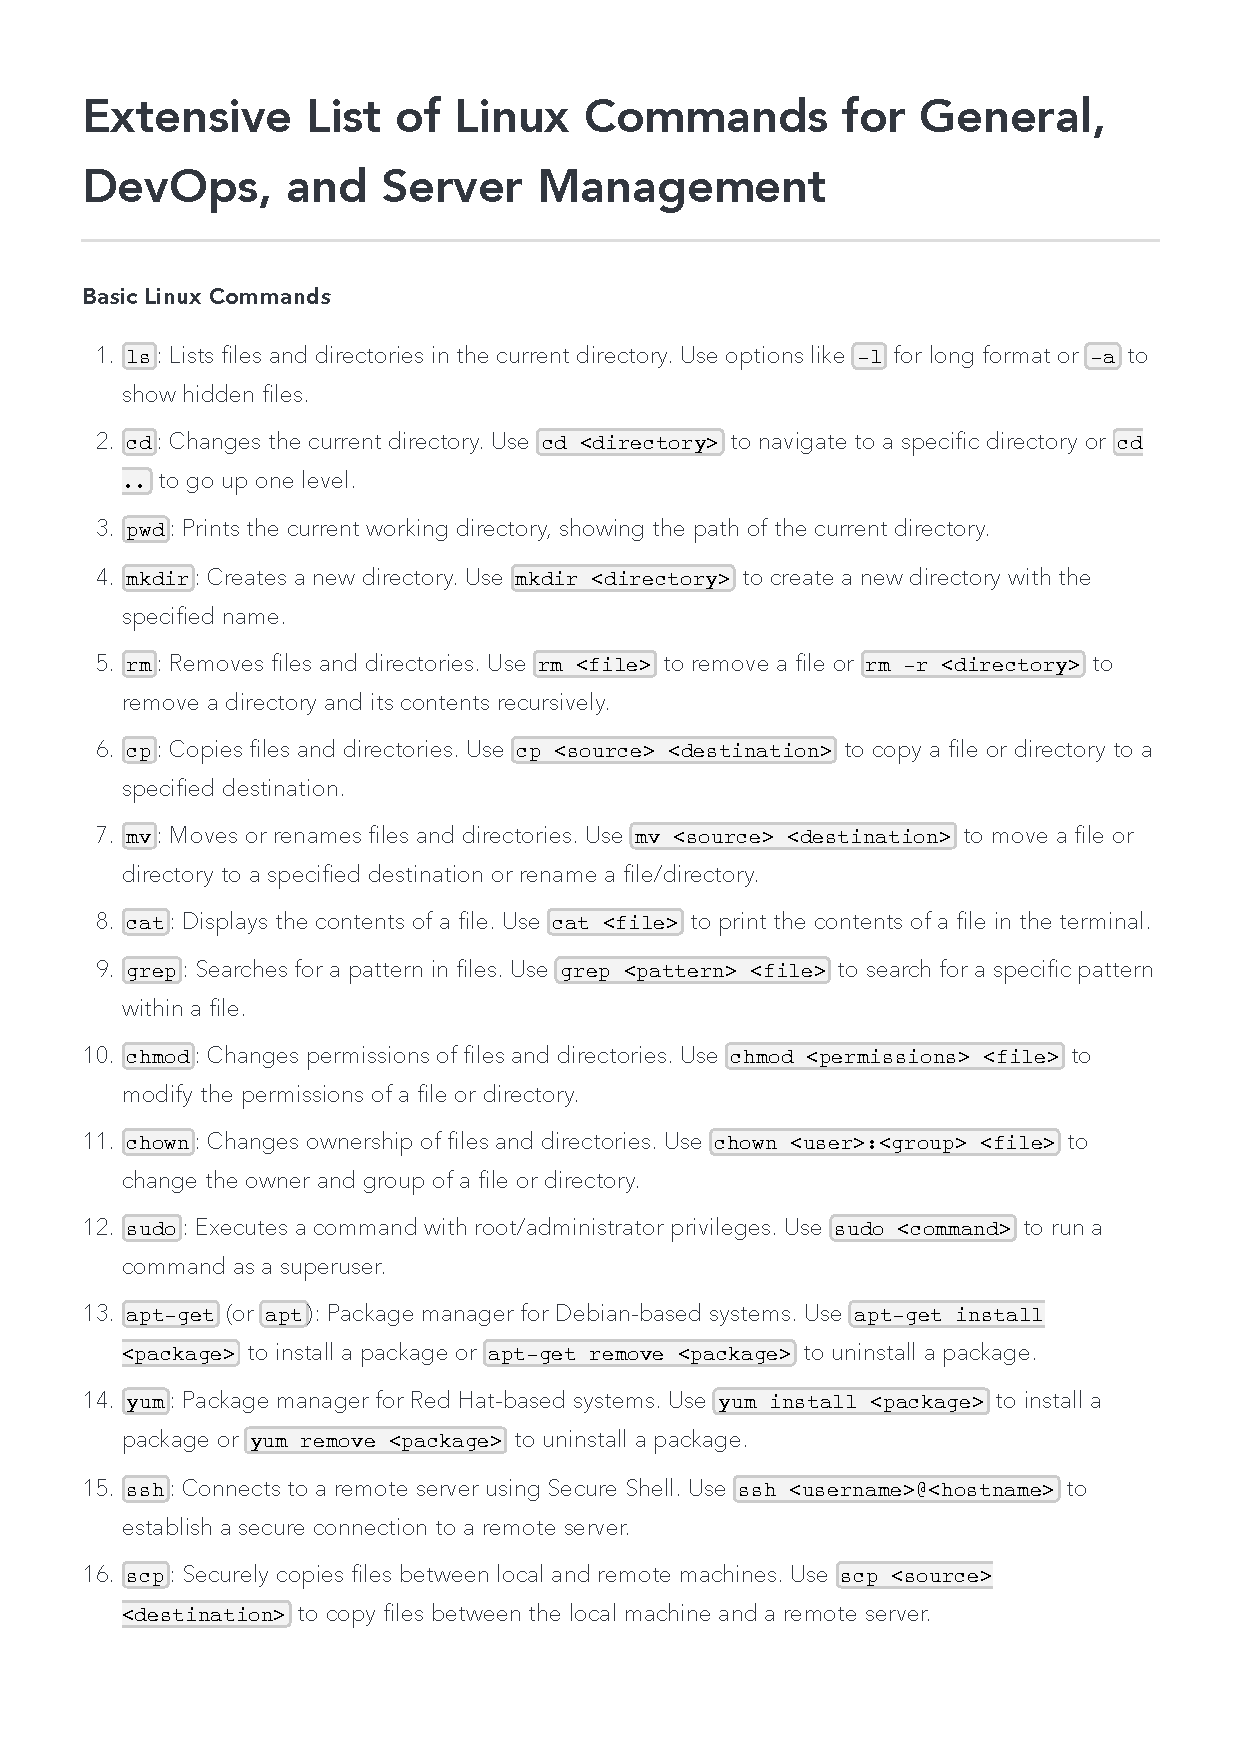
\includepdf[pages=-]{Assets/Extensive-List-of-Linux-Commands-for-General-DevOps-and-Server-Management.pdf}

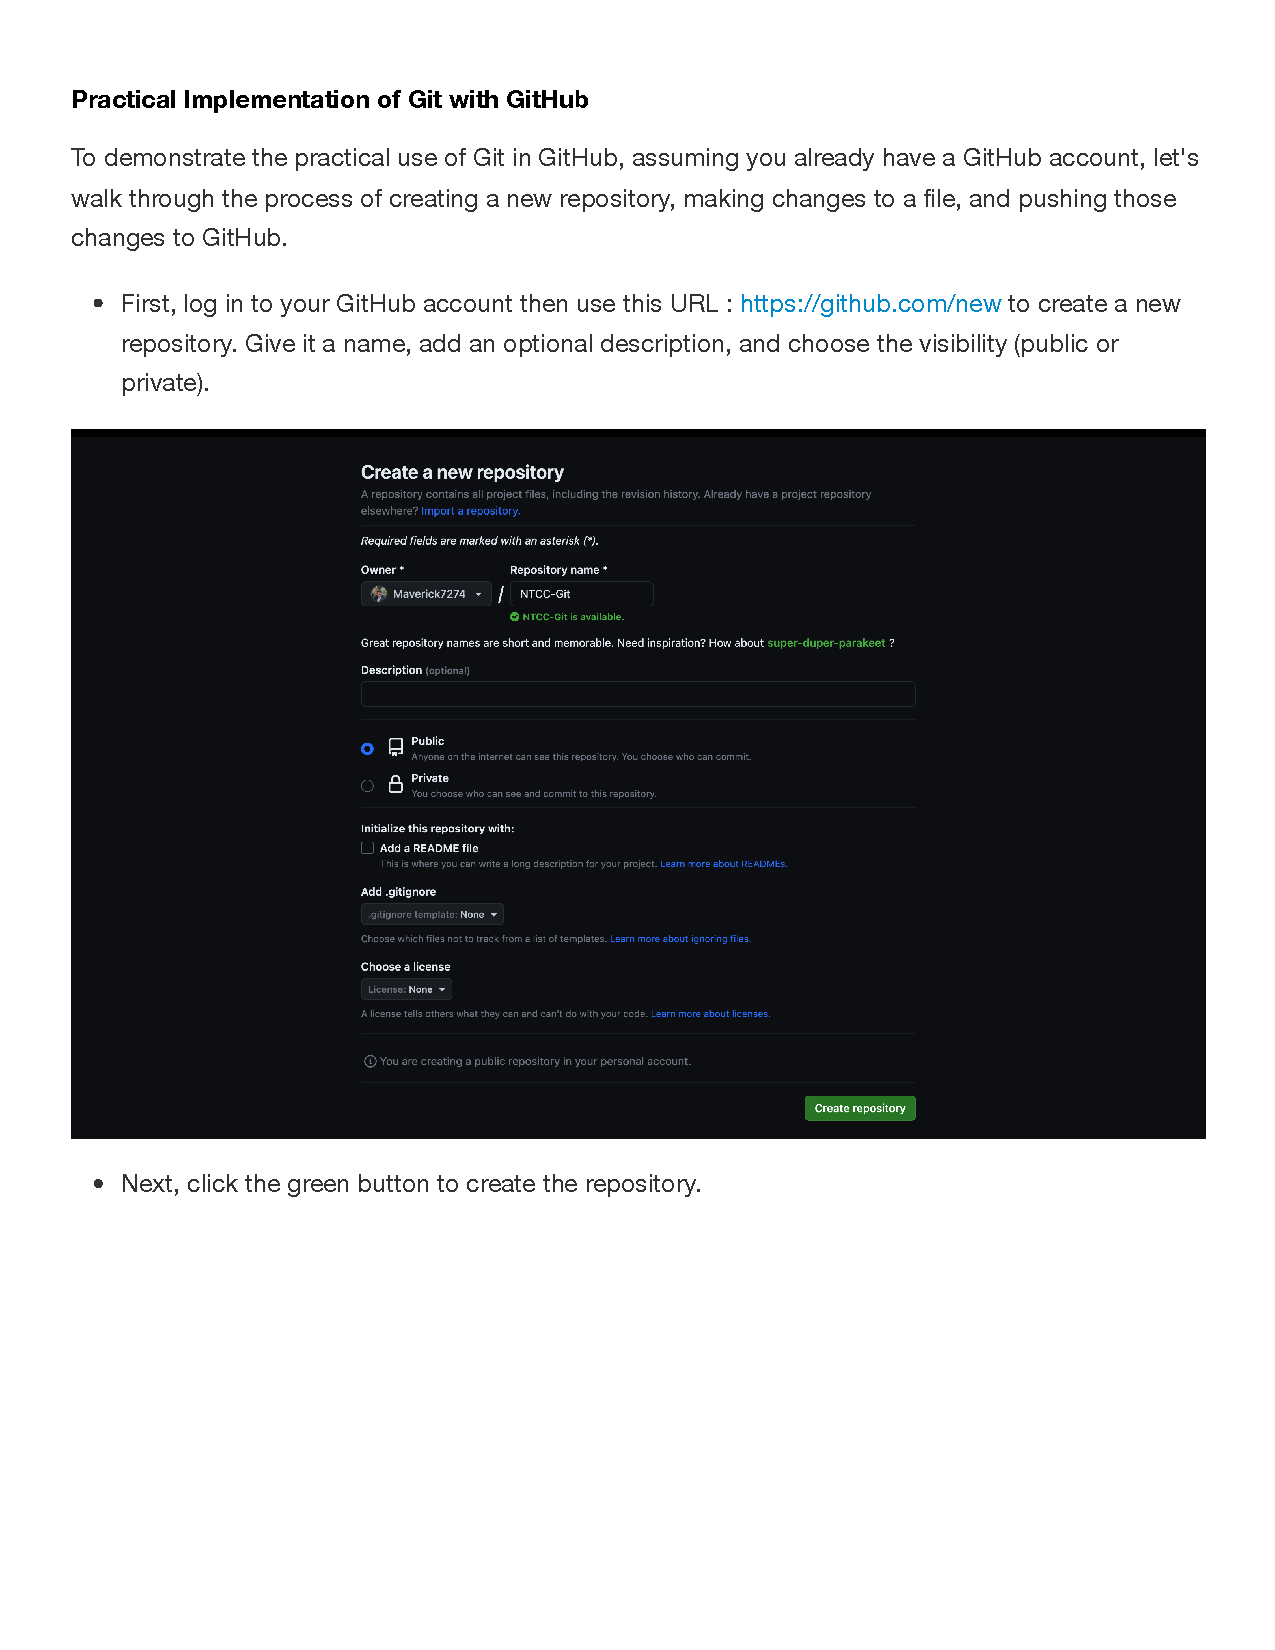
\includepdf[pages=-]{Assets/git.pdf}

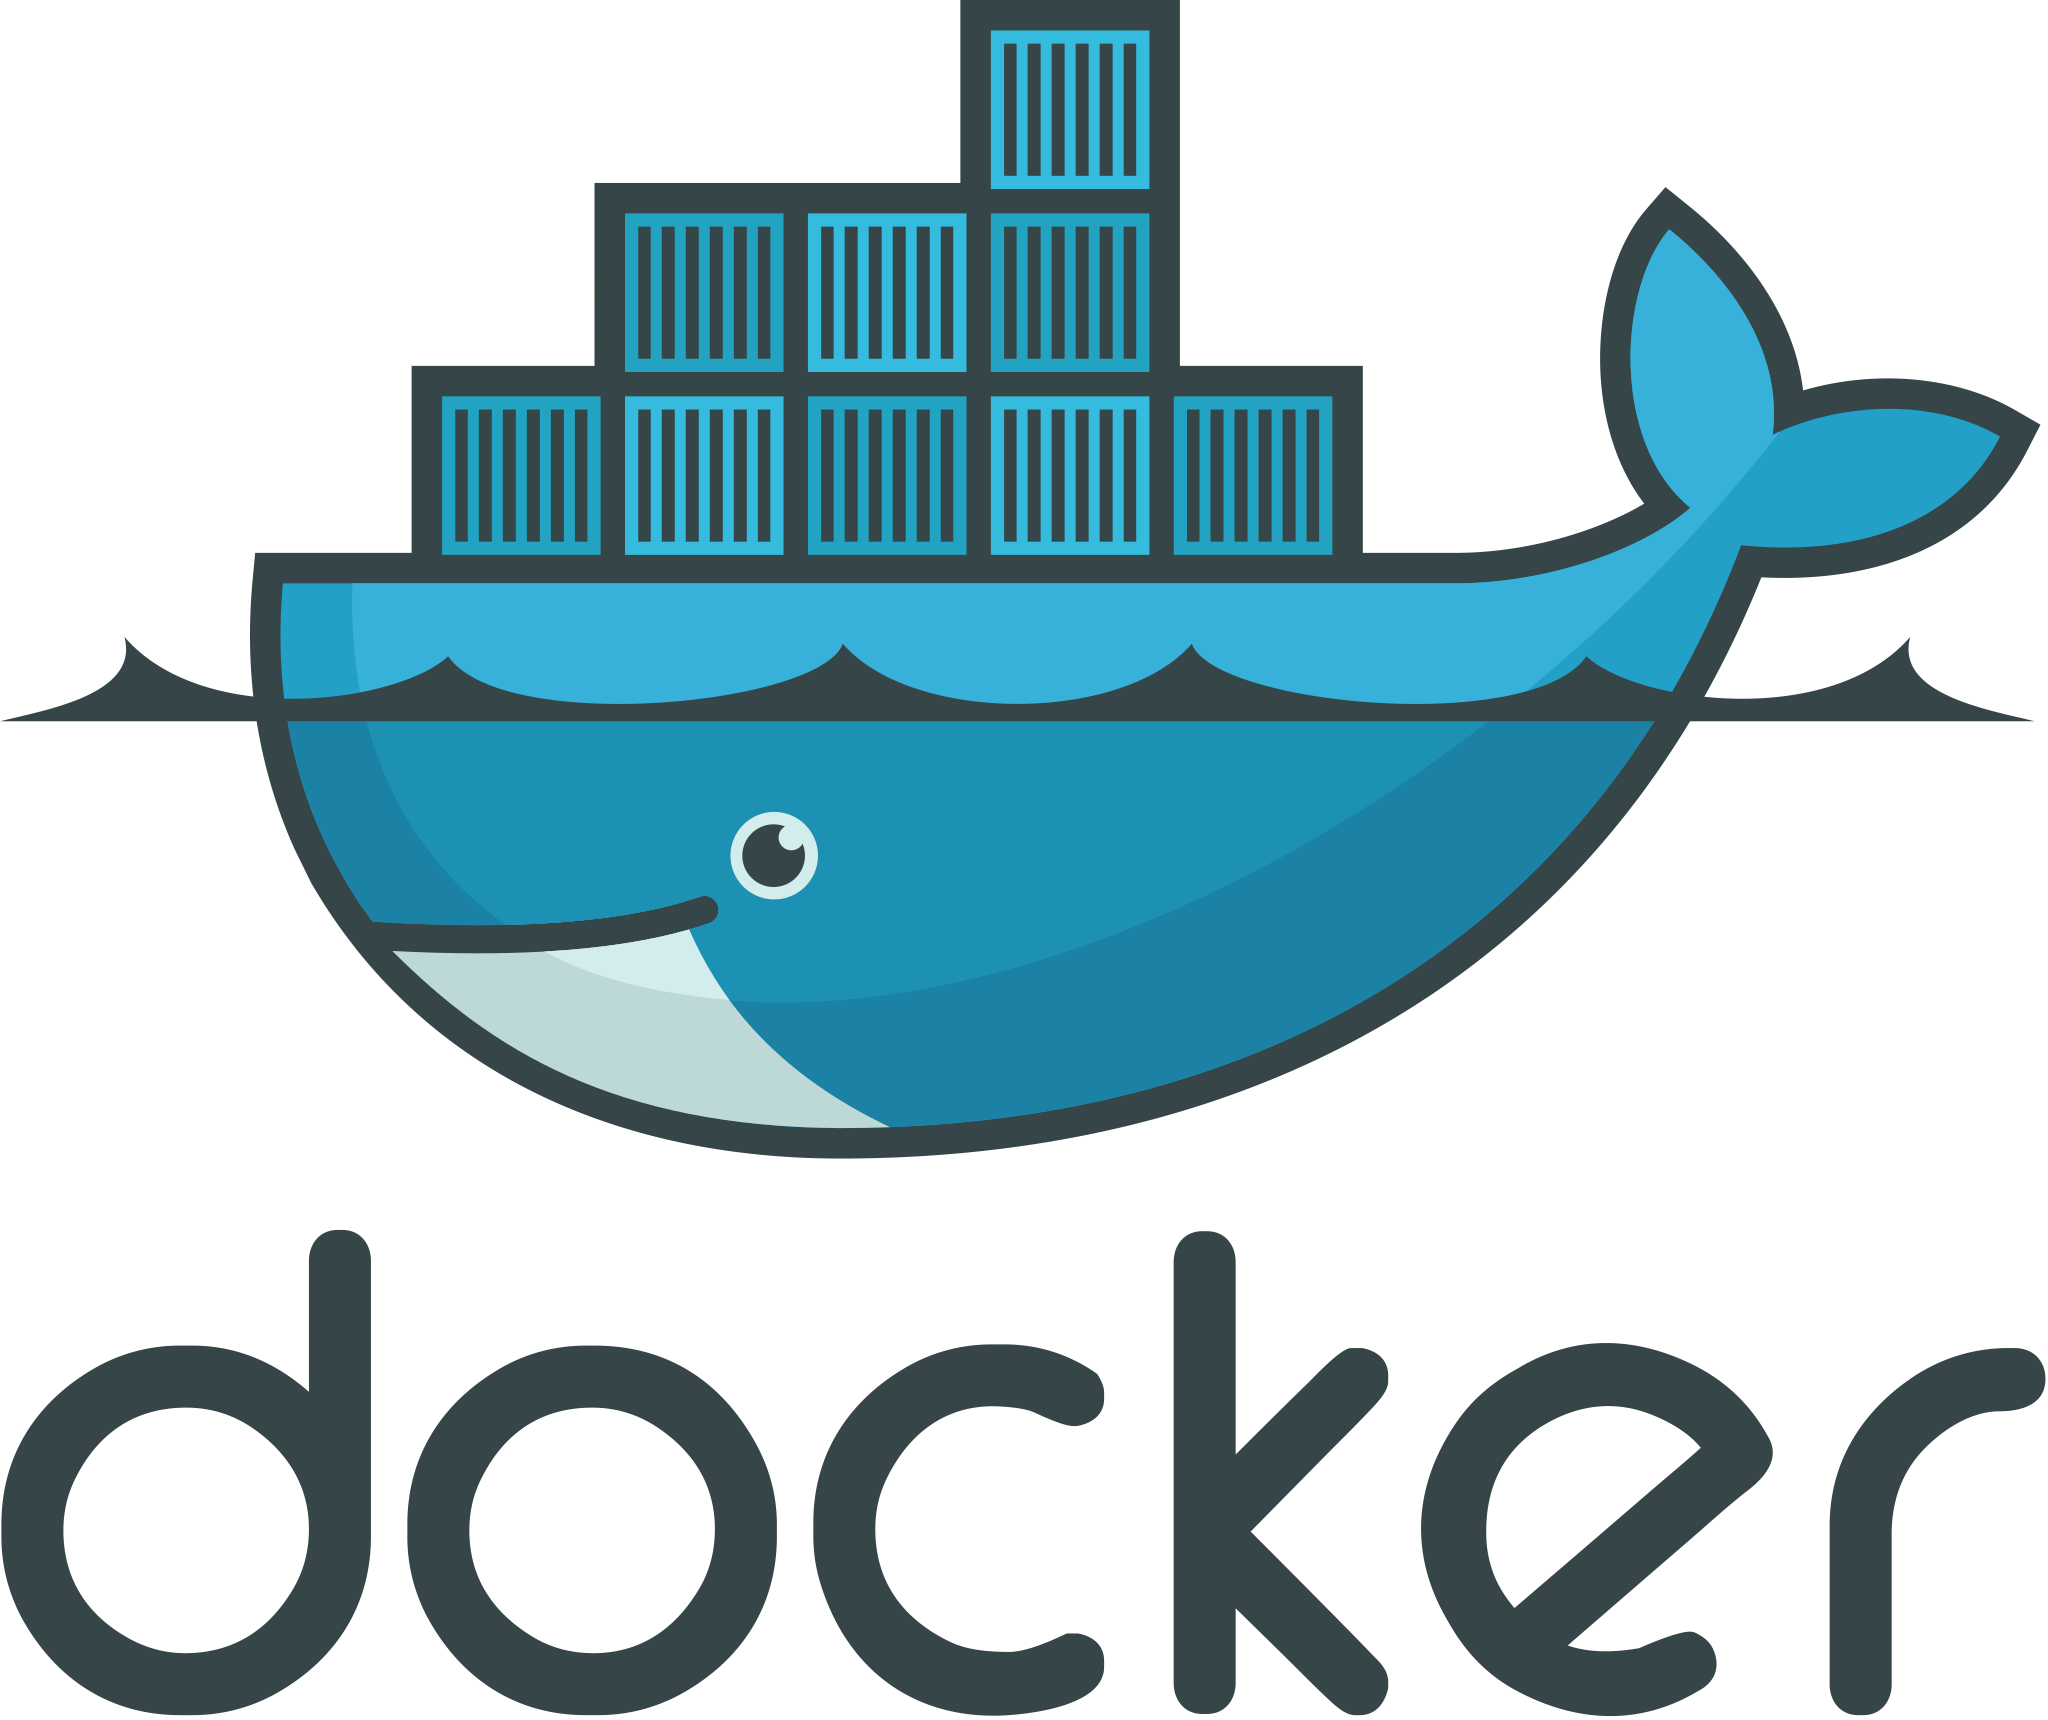
\includepdf[pages=-]{Assets/docker.pdf}